\begin{fact}
	$\forall (a;b) \in \big( \RRsp \big)^2$,
	$\ln(a b) = \ln a + \ln b$.
\end{fact}


\begin{proof}
	Par définition de $\ln$, nous avons 
	$\ln(a b) = \ln a + \integrate*{\frac1t}{t}{a}{ab}$.
	Concentrons-nous sur $I_{a}^{ab} = \integrate*{\frac1t}{t}{a}{ab}$.
	Pour cela, notons $\setproba{L}$ la représentation graphique  de $\ln$.
	
	\begin{center}
		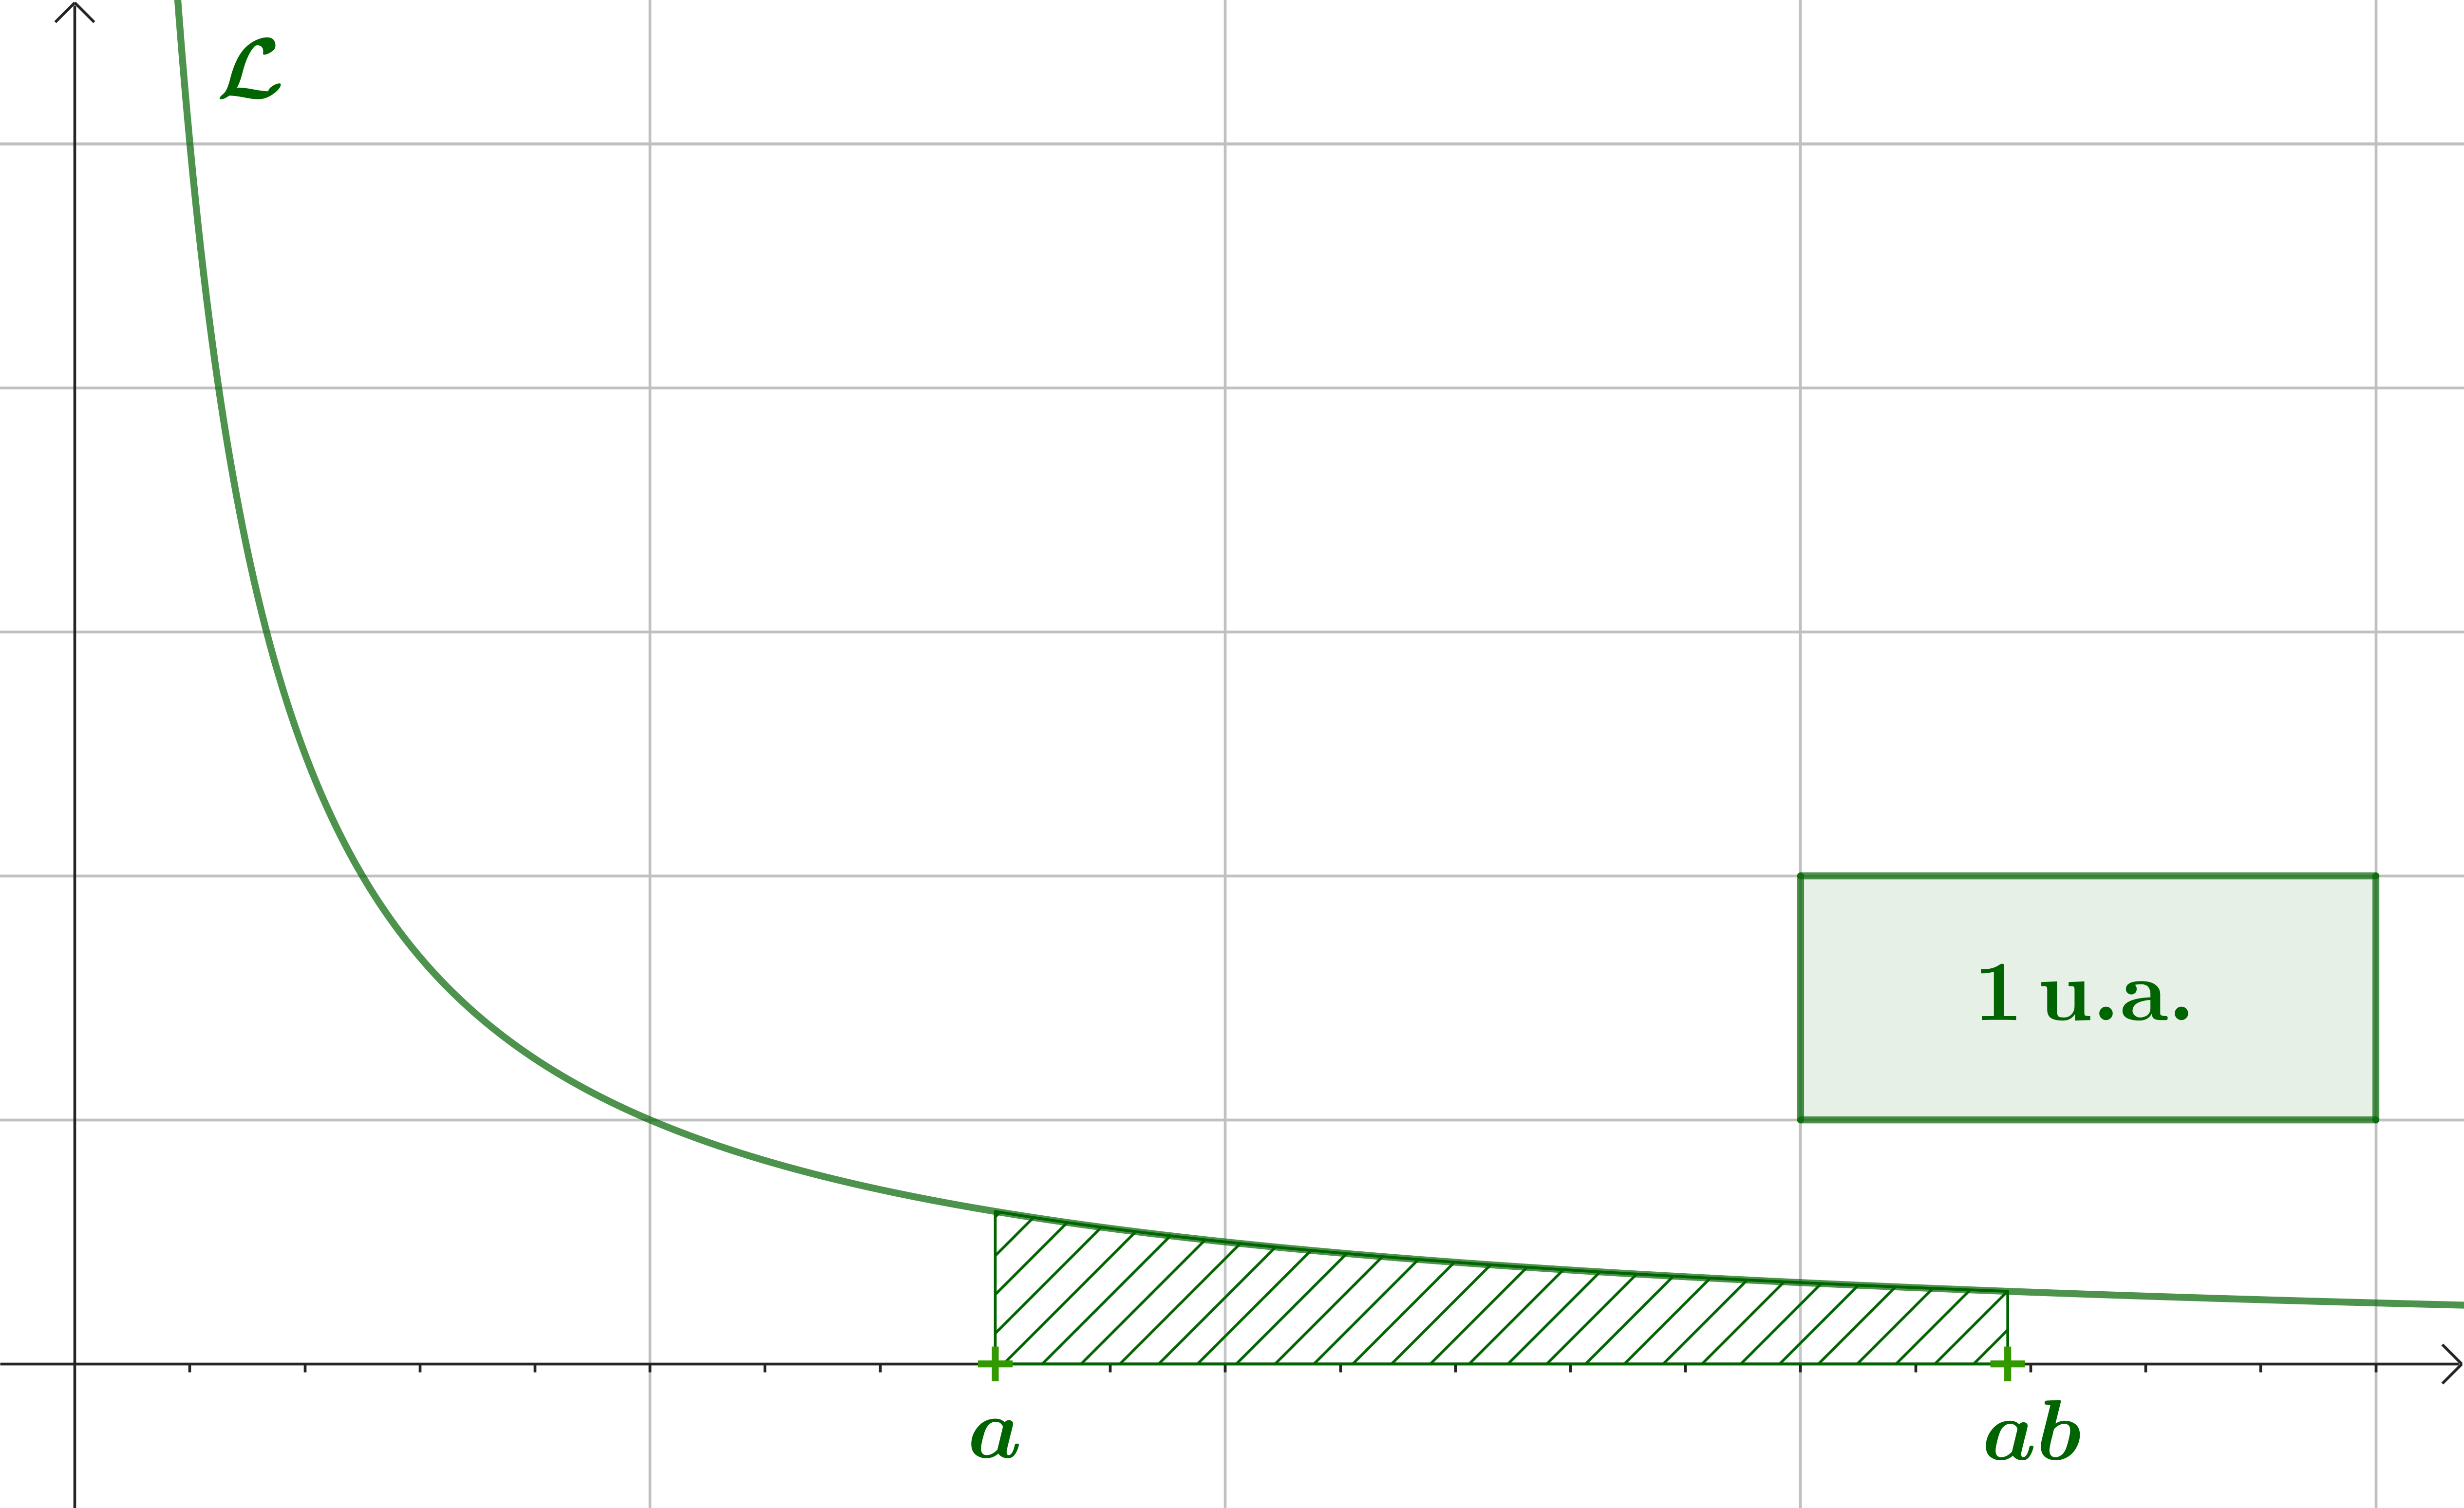
\includegraphics[scale=.5]{content/ln/func-eq-1.png}
	\end{center}

	Une dilatation horizontale $\phi$ de coefficient $\frac1a$ transforme $M(x_M ; y_M)$ en $M^{\,\prime}\big( \frac{x_M}{a} ; y_M)$. 
	Appliquons $\phi$ à la surface hachuré associée à l'intégrale $I_{a}^{ab}$, ainsi qu'à la fonction $\ln$ qui devient $f: x \mapsto \frac{1}{a x}$, puisque nous devons avoir $f(\frac{x}{a}) = \ln x$. 
	Il est important de noter qu'un rectangle d'une unité d'aire est transformé par $\phi$ en un rectangle de $\frac1a$ unité d'aire.

	\begin{center}
		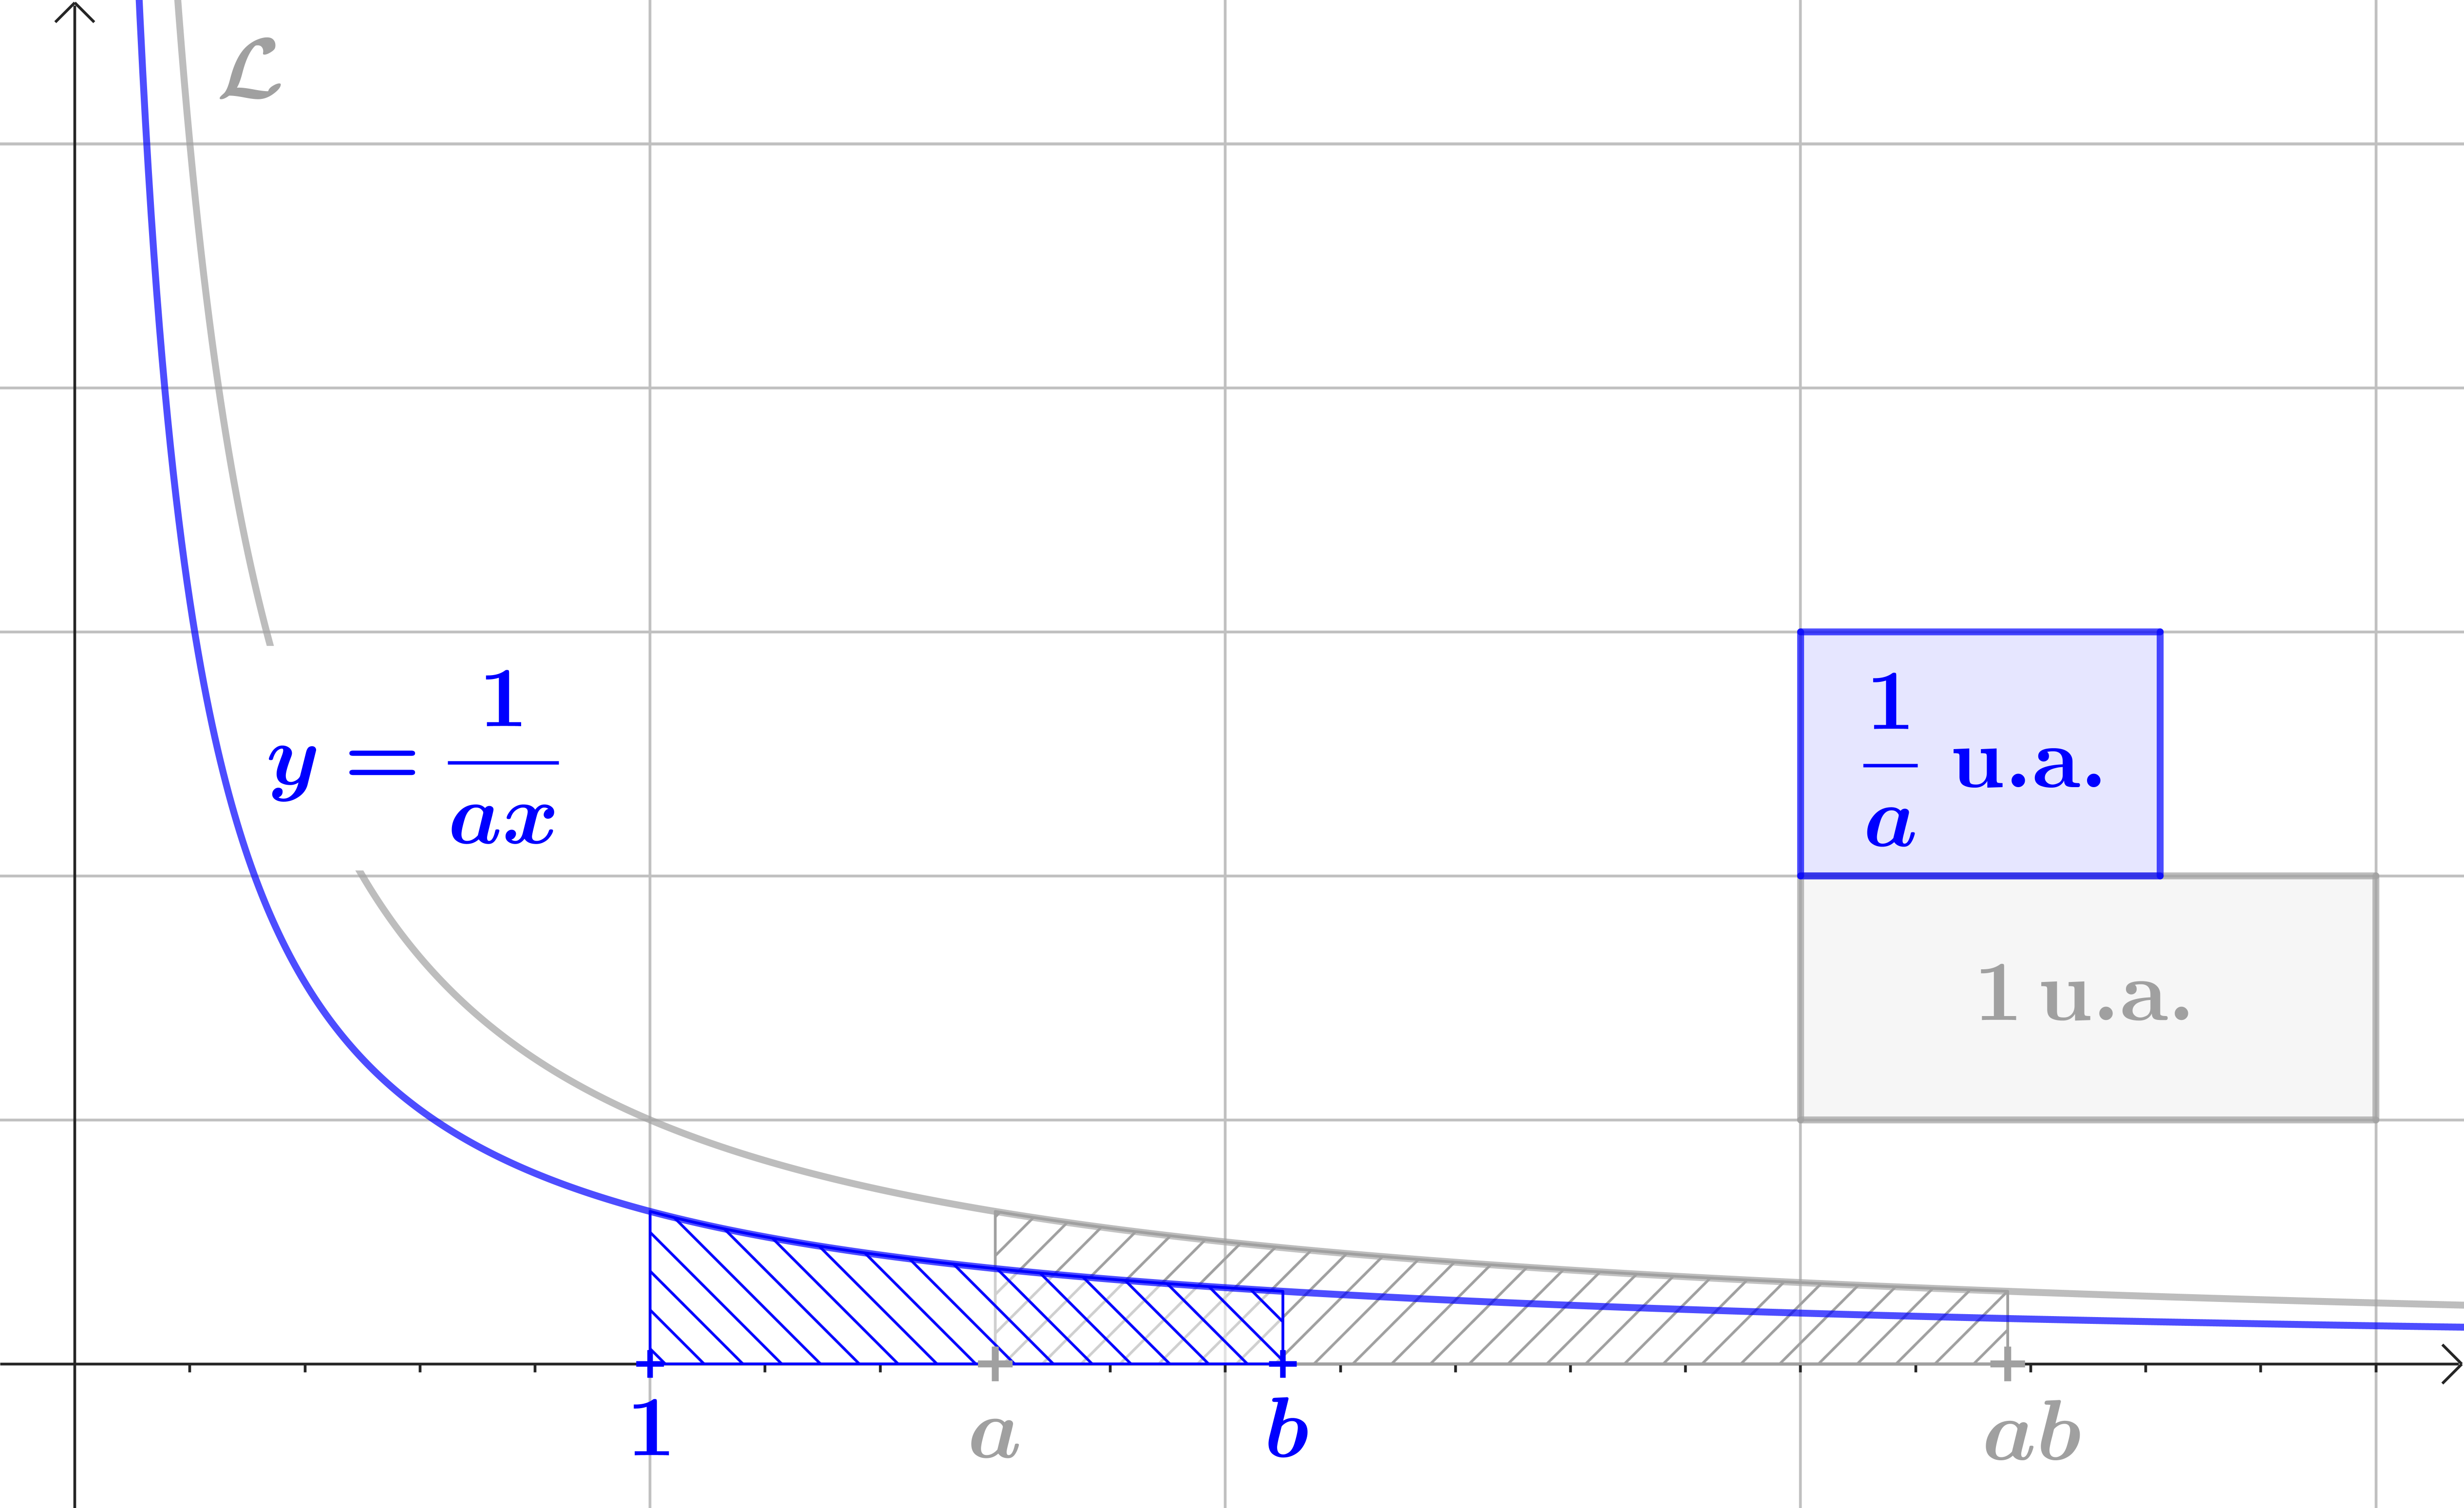
\includegraphics[scale=.5]{content/ln/func-eq-2.png}
	\end{center}

	Une dilatation verticale $\psi$ de coefficient $a$ transforme $M(x_M ; y_M)$ en $M^{\,\prime}\big( x_M ; a y_M)$. 
	Appliquons $\psi$ à la surface hachuré associée à l'intégrale $\integrate*{\frac{1}{at}}{t}{1}{b}$, ainsi qu'à la fonction $f$ qui devient la fonction $\ln$. Notons qu'un rectangle de $\frac1a$ unité d'aire est transformé par $\psi$ en un rectangle d'une unité d'aire.

	\begin{center}
		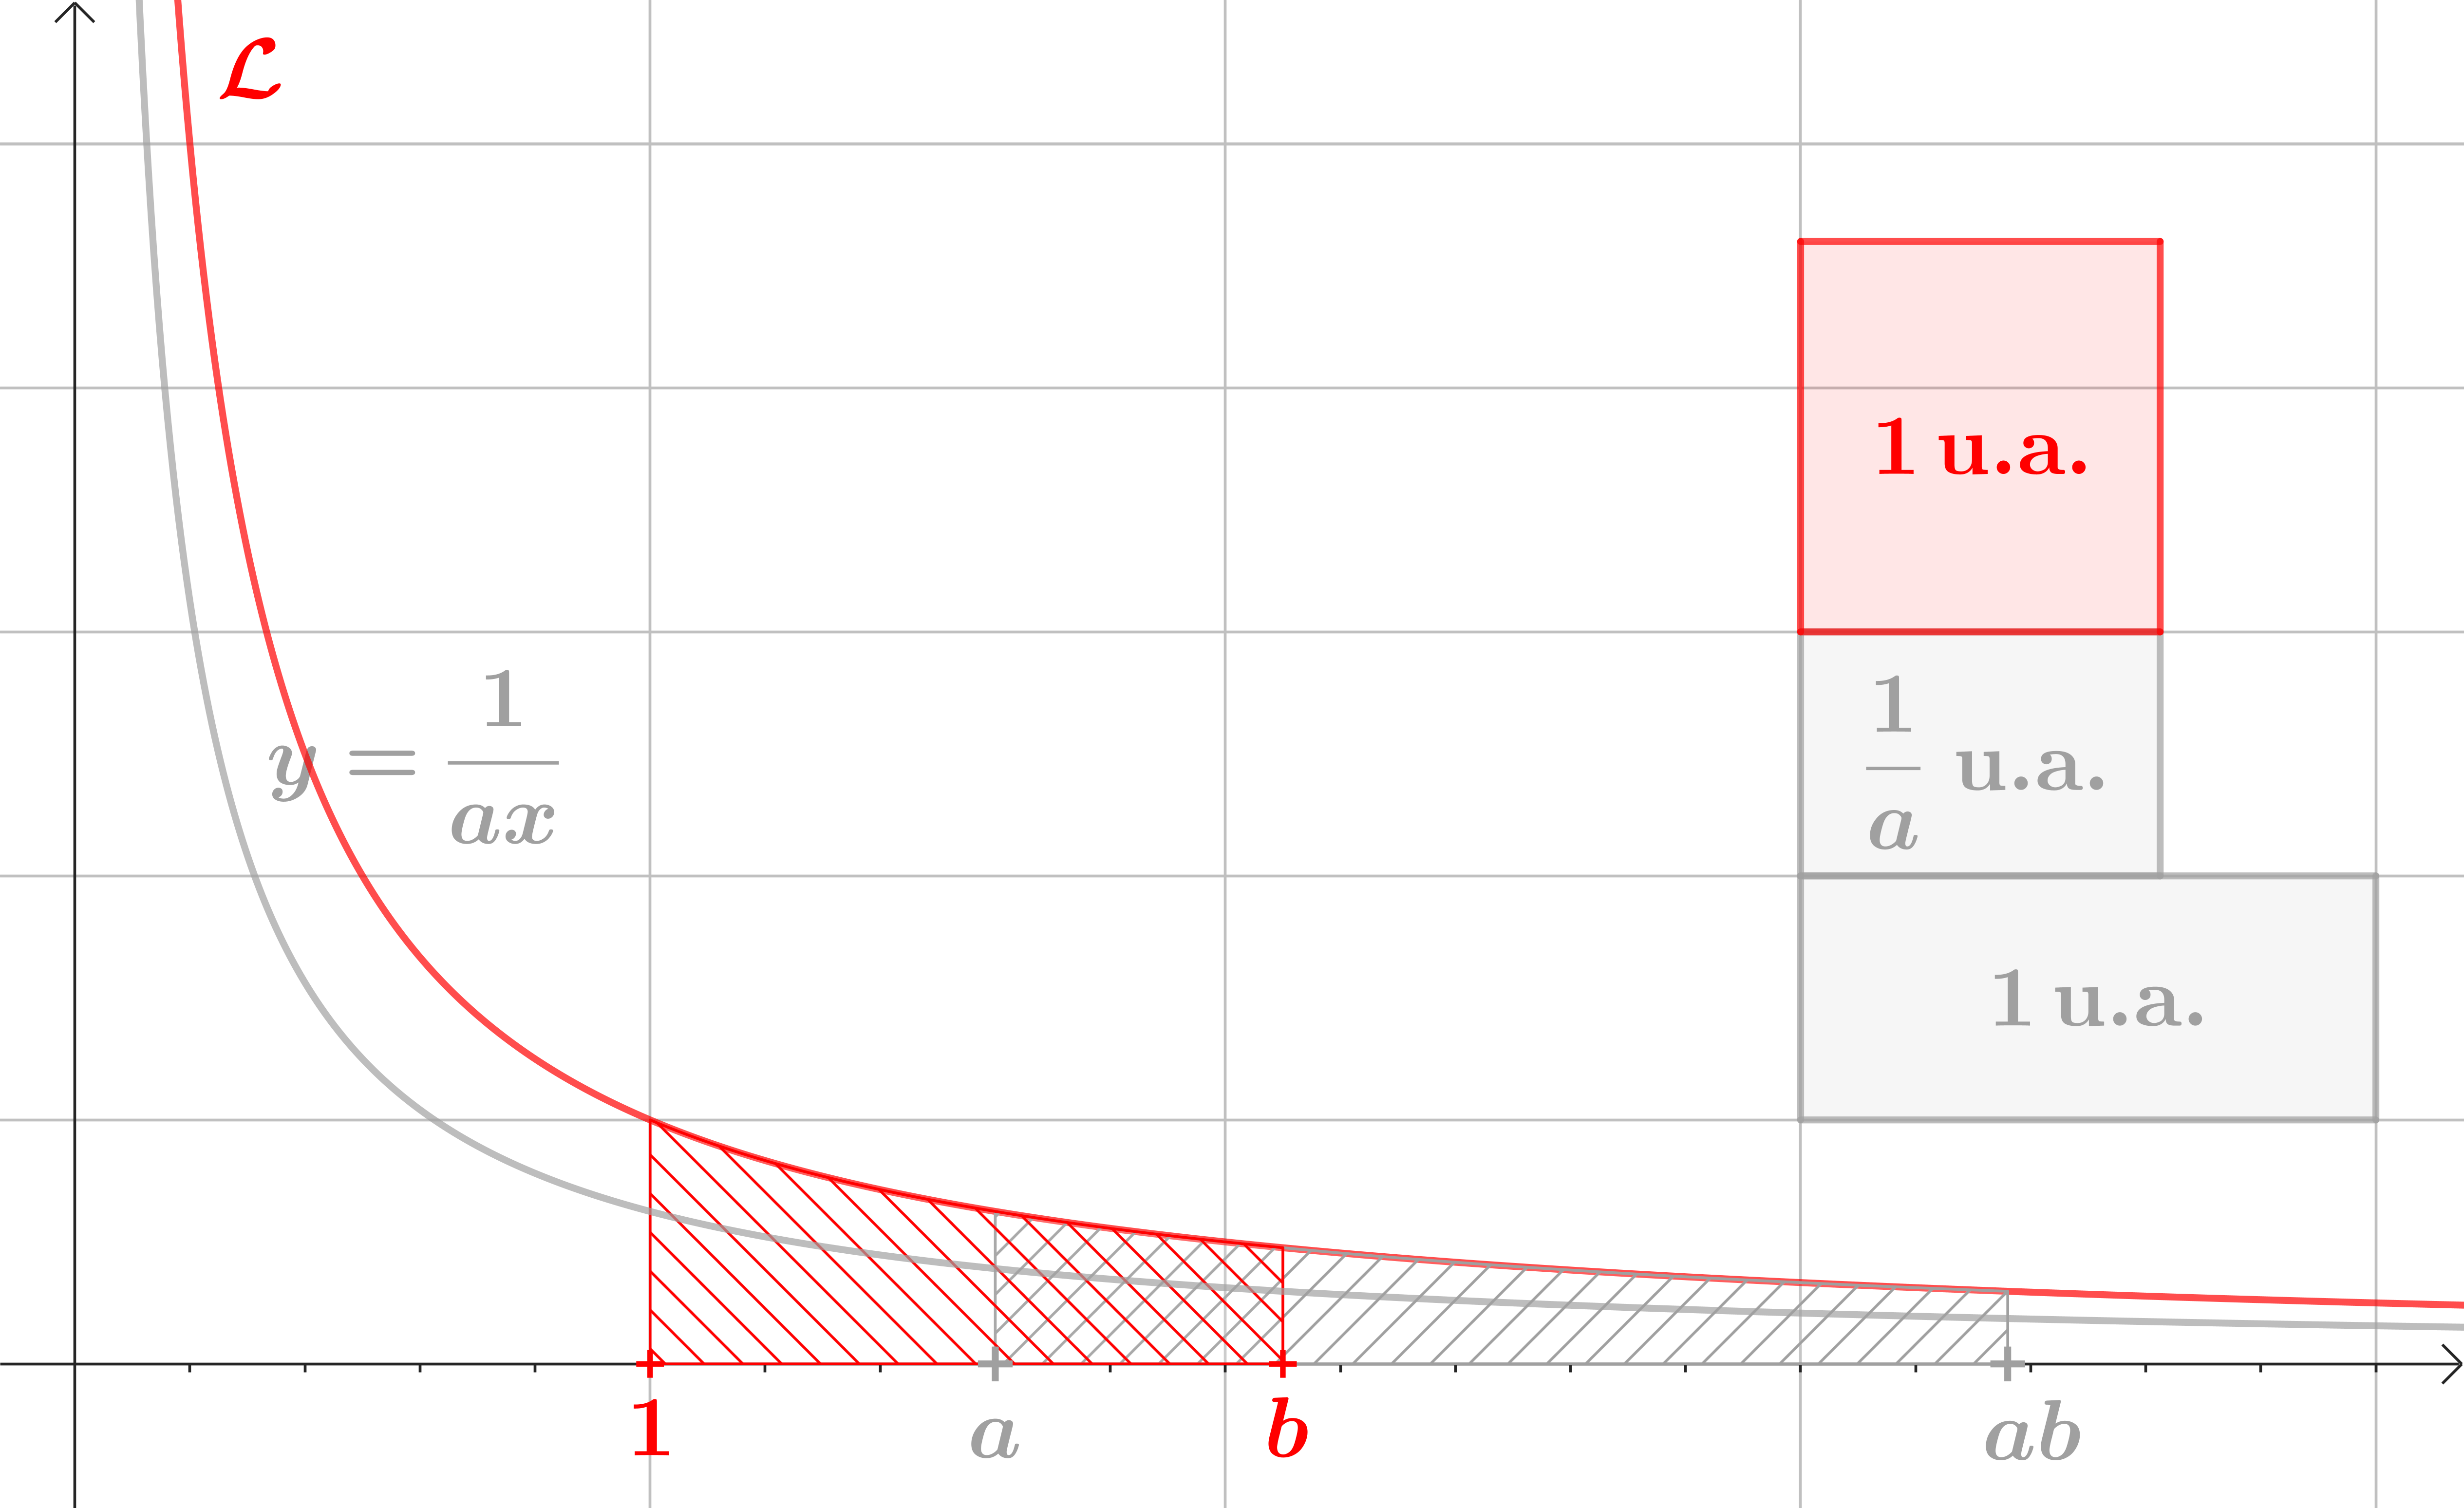
\includegraphics[scale=.5]{content/ln/func-eq-3.png}
	\end{center}
	
	Nous venons de justifier que $I_{a}^{ab} = \integrate*{\frac{1}{t}}{t}{1}{b}$,
	d'où $\ln(a b) = \ln a + \ln b$ comme annoncé.
\end{proof}

